\documentclass{article}
\usepackage{graphicx}
\usepackage{amsmath,amssymb,amsthm}
\usepackage{color}

\usepackage{algpseudocode}
\usepackage{algorithm}
%\usepackage{minted}

\DeclareMathOperator*{\argmax}{arg\,max}
\DeclareMathOperator*{\argmin}{arg\,min}

\begin{document}

\title{Review Notes on Dead End Elimination(DEE)}

\author{Subhodeep Moitra \\ {\tt subho@cmu.edu}}

\maketitle

\begin{abstract}
The Dead-End Elimination(DEE) algorithm is a technique for pruning the search space for discrete combinatorial optimatization problems. It has traditionally been applied to several problems in computational structural biology such as side chain placement and protein design. It works by provably eliminating candidates that cannot be part of the global minimum energy conformation(GMEC). There are a number of different DEE criteria and they have different eliminating power, computational costs an applications. In this review we present the major DEE criteria, intuition of why it works and also new research ideas. 
\end{abstract}

\section{Introduction}
Some problems in computational structural biology such as sequence design or side chain rotamer optimization can be posed as discrete combinatorial optimization problems. These problems are more formally defined in the following section. Meanwhile, we will use the side chain optimization problem as a running example since the sequence design problem is conceptually the same.  In these problems we try to minimize an energy function parametrized by the discrete variable. The global minumum of the energy function is known as the GMEC (Global Minimum Energy Conformation). Finding the GMEC is NP-hard as shown by~\ref{Pierce}. This is a sobering result and efforts to find a polynomial time solution for these protein design problems is likely to be fruitless. Nevertheless, the nature of the rotamers or the sequences is such that some of these states are clearly wrong and can be safely ignored while searching for the GMEC. For e.g.(1) a rotameric position which causes clashes with the backbone can be safely ignored from consideration (2) a polar amino acid can be safely ignored from the hydrophobic core. This leads us to the Dead-End Elimination algorithm (DEE). 
\\
\\
The DEE algorithm has been used as a search space reduction technique for problems in computational structural biology. These problems involve an exponential number of possible solution candidates. The DEE algorithm is able to successfully prune the search space while retaining the GMEC. The basic idea  is to be able to find bad combinations of variables known as dead ends. This is in direct contrast to the Dynamic programming style of finding a solution, which involves keeping the best and most promising candidates. 
\\
\\
Every DEE algorithm essentially has the following components :
\begin{enumerate}
\item A well defined set of discrete independent variables
\item A \emph{precomputed} numerical value(considered the energy) associated with each element in the set of variables. You can even define these energies for their pairs, triples, etc
\item A criterion for determining when an element is a dead end
\item An objective function considered to be the energy function to be minimized
\end{enumerate}

The energy function has pairwise energy terms for a reason. This relative merits of a candidate rotamer at a particular position is evaluated using only the contributions from the unit and the pairwise energy terms and not the total energy of all conformations in all positions. By evaluating the relative energy contributions of energy of the candidates rotamers for the position under consideration it is possible to ascertain incompatibility with GMEC without knowing the actual minimum energy. The combinatorial cost of this procedure is far less than actually enumerating the entire space in order to find the GMEC. 
\\
\\
The DEE algorithm has undergone a lot of change since it was first published~\cite{Desmet1992} in 1992. Newer criteria for the pruning the search space emerged. Newer criteria are measured by their efficiency i.e. how quickly you can check criterion and the eliminating power i.e. how much of the space they can prune. Stronger criteria were added that were able to prune out more of the search space. A number of novel criteria and DEE models emerged that are able to do some non-traditional DEE tasks such as Backrub modeling, flexible backbone, continuous rotamers etc. The DEE algorithm is no magic bullet. Even though it is typically able to prune the search space of protein problems effectively, the exhaustive search to be performed afterwards can still be quite computationally demanding.

\subsection{Side chain placement problem}
The side chain placement problem(SCP) refers to finding the conformation of the side chains of the protein assuming a fixed backbone. The entire continuous space of the side chains is not modelled. They are usually discretized into a set of discrete rotamers~\ref{Dunbrack}. Every conformation has an associated energy. The energy function is decomposable into energy contributions from each of the individual amino acids or pairs of amino acids. This is reasonable since atoms in proteins are assumed to interact only by two body potentials. The energy of particular conformation represented by a vector $r$ is represented as : 
\[
E(r) = \sum_{i=1}^{N}E_i(r_i) + \sum_{i<j}E_{ij}(r_i,r_j)
\]

where $E(r)$ corresponds to the overall energy of a rotamer conformation space represented by the vector $r$. The rotamer for amino acid $i$ is represented by $r_i$. Also, $r_i^A$ corresponds to the rotamer at position $i$ taking state A. The rotamers for a particular amino acid are restricted to a discrete set $r_i \in \{1,2,\cdots,R_i\}$. $E_i(r_i)$ corresponds to the precomputed energies for rotamer for amino acid $i$ and the backbone. $E_{ij}(r_i,r_j)$ corresponds to the precomputed energies between the pair of rotamers for amino acid $i$ and $j$ respectively. 
Note that, $E_{kk}(r_k^A,r_k^A)$ that the pair energy between a rotamer and itself is taken to be zero. This simplifies description of the pairs criterion to be presented below. 
\\
\\
In principle one can make energy function arbitrarily complex taking contributions from tuples of amino acids. However the fact the function decomposes into atomic parts is what makes it possible to apply pruning techniques such as DEE.  The side chain placement problem is a discrete combinatorial optimization problem which involves finding the conformation $r^*$ which minimizes the function $E(r)$. This conformation $r^*$ is known as the global minimum energy conformation or the GMEC.
\[
\begin{split}
r^* &= \argmin_{r_i \in \{1,2,\cdots,R_i\}} E(r) \\
&= \argmin_{r_i \in \{1,2,\cdots,R_i\}} \sum_{i=1}^{N}E_i(r_i) + \sum_{i<j}E_{ij}(r_i,r_j)
\end{split}
\]
This problem has been recast into a number of different frameworks such as Integer programming, graph based methods, etc. Nevertheless, this problem has been shown to be NP-Hard~\ref{Pierce}. There are a number of methods that try to solve the problem with no guarantees for optimality using techniques such as simulated annealing, monte carlo optimization, etc.  The state of the art is the SCWRL4~\ref{SCWRL4} algorithm. SCWRL4's goal is performance rather than algorithmic novelty. So they use a number of different existing successful techniques in order to find a good placement. 
\\
\\
The DEE algorithm can be used in those algorithms that try to exactly find the GMEC. Basically, any algorithm that attempts to find the GMEC has to resort to exhaustive search unless there is some structure in the energy function. But most SCP problems do not have this kind of structure and can have exponential worst case behavior. DEE is used to prune the search space. The original DEE algorithm~\ref{Desmet92} used the singles and the doubles elimination criteria for pruning single and pairwise rotamer pairs. 


\subsection{Protein Design problem}
The protein design problem(PD) refers to finding an amino acid sequence that is compatible with a desired protein structure. The compatibility with the desired structure is measured through an energy function. The form of the energy function is much like the side chain placement problem. The optimization problem becomes a discrete combinatorial optimization problem. The optimization over the sequence space hides an inner optimization of the rotameric space
\[
\begin{split}
S^* &= \argmin_{S} E^*(S) \\
	&= \argmin_{S} \left( \min_{r} E(r) \right) \quad \text{s.t. $\tau(r)=S$} \\
	&= \argmin_{S} \left( \min_{r_i \in \{1,2,\cdots,R_i\}} \sum_{i=1}^{N}E_i(r_i) + \sum_{i<j}E_{ij}(r_i,r_j) \right) \quad \text{s.t. $\tau(r)=S$}
\end{split}
\]

Here, $E^*(S)$ corresponds to the minimum energy rotameric conformation given a particular sequence. $\tau(r)$ is a mapping from a rotamer space to a sequence. This has an implicit minimization which is the same as finding the GMEC for the SCP problem. The backbone is held fixed regardless of the amino acid sequence or the position of the rotamers. This is  ofcourse not a realistic assumption, but it is done so by design. The goal is to have a protein sequence which assumes the backbone shape, not just to find a stable structure. The PD problem can in fact be reformulated into the SCP problem by extending the rotameric space. The optimal sequence is then trivially retrieved by mapping the rotamers to their corresponding amino acids.
\[
\begin{split}
S^* &= \tau\left( \min_{r_i \in \{1,2,\cdots,R_{all}\}} \sum_{i=1}^{N}E_i(r_i) + \sum_{i<j}E_{ij}(r_i,r_j) \right)
\end{split}
\]
where $R_{all}$ corresponds to all the rotamers of all the amino acids. In practice, we do not need to search over all positions in the protein. We are most often interested in redesigning an active site or a binding site. We also don't need to search over the space of all the amino acids at a particular position. Knowledge about the hydrophobicity and/or evolutionary constraints can help restrict the search space apriori. 


The DEE algorithm can be used here again to significantly reduce the search space. A short zinc finger protein was redesigned using an early version of the DEE algorithm~\ref{Dahiyat1997}. 

\section{Original Criteria}
The original DEE algorithm~\cite{Desmet1992} proposed single as well as multi-residue rotamer criteria. They are as follows :

\subsection{Singles Elimination criterion}
The rotamer $r_i^A$ is a dead end if there exists another rotamer $r_i^B$ for amino acid $i$ and the following condition holds: 
\begin{equation}	
\label{Singles:criteria} 
E_i(r_i^A) + \sum_j \min_X E_{ij}(r_i^A,r_j^X) > E_i(r_i^B) + \sum_j \max_X E_{ij}(r_i^B,r_j^X) \quad   ; j\neq i
\end{equation}
This basically, says that if the best possible energy contribution by the rotamer $r_i^A$ is worse than the worst possible energy contribution by another rotamer $r_i^B$, letting the rotamers of other amino acids be anything, then $r_i^A$ is a dead-end and should be eliminated.
This criterion appears to scale as $O(n^2r^3)$ where $r$ represents all the rotamers for all the amino acids in the protein and $n$ is the length of the protein. However, we can achieve a $O(n^2r^2)$ computational cost by computing the left hand side and the right hand side separately and storing the results~\cite{Pierce2000}.

\subsection{Pairs Elimination criterion}
The pairs elimination criterion generalizes the singles elimination criterion by allowing the elimination of rotamer pairs. This can be extended to multi-residue combinations as well. To illustrate this criterion we will introduce the following notation. The self-energy of a pair of rotamers is described as : 
\[
\mathcal{E}(r_i^A,r_j^P) = E_i(r_i^A) + E_j(r_j^P) + E_{ij}(r_i^A,r_j^P)
\]
A rotamer pair $(r_i^A,r_j^P)$ is a dead-end if there exists another amino acid pair $(r_i^B,r_j^Q)$ such that the following condition holds:
\[
\begin{split}
\mathcal{E}(r_i^A,r_j^P) &+ \sum_k \min_X \left( E_{ik}(r_i^A,r_k^X) + E_{jk}(r_j^P,r_k^X) \right) > \\ & \mathcal{E}(r_i^B,r_j^Q) + \sum_k \max_X \left( E_{ik}(r_i^B,r_k^X) + E_{jk}(r_j^Q,r_k^X) \right) \\
& \text{where $k\neq j \neq i$}
\end{split}
\]
This criterion scales $O(r^3)$ where $r$ represents all the rotamers for all the amino acids in the protein. More generally, for multi-residue criteria of order $m$ it scales as $O(r^{m+1})$. 

\subsection{Proof of Singles DEE criterion}
The main idea behind the DEE criteria is local optimality. It means that at GMEC, each residue has a locally optimal assignment. i.e. it is not possible to substitute any other rotamer type for that residue given that the others are in GMEC. Now on to the proof.
\\
\\
The optimality of GMEC means that 
\begin{equation}
\label{Singles:opt}
E(r^*) \leq E(r) \quad \forall r
\end{equation}
Let us expand the energy function focusing on a rotamer $r_i^G$ in GMEC. $G$ represents a rotamer in GMEC.
\begin{equation}
\label{Singles:gmec}
E(r^*) = E_{bb} + E_i(r_i^G) + \sum_j E_{ij}(r_i^G,r_j^G) + \sum_j E_j(r_j^G) + \sum_{j<k} E_{jk}(r_j^G,r_k^G) \quad ; j,k\neq i
\end{equation}
Now, let us suppose that our residue of interest $r_i$ adopts a different rotameric conformation from  GMEC such as $r_i^T$. The energy is represented as :
\begin{equation}
\label{Singles:nongmec}
E(r) = E_{bb} + E_i(r_i^T) + \sum_j E_{ij}(r_i^T,r_j^G) + \sum_j E_j(r_j^G) + \sum_{j<k} E_{jk}(r_j^G,r_k^G) \quad ; j,k\neq i
\end{equation}
Applying the GMEC optimality criteria from equation~\ref{Singles:opt} and combining equations \ref{Singles:gmec} and \ref{Singles:nongmec}, we get the \emph{local optimality criterion}. 
\begin{align*}
E_i(r_i^G) + \sum_j E_{ij}(r_i^G,r_j^G) \leq E_i(r_i^T) + \sum_j E_{ij}(r_i^T,r_j^G)  \quad   
; j\neq i 
\end{align*}



Taking mins and maxs on the LHS and RHS still preserves the inequality. We get, 
\begin{equation}
E_i(r_i^G) + \sum_j \min_X E_{ij}(r_i^G,r_j^X) \leq E_i(r_i^T) + \sum_j \max_X E_{ij}(r_i^T,r_j^X)  \quad   
; j\neq i 
\end{equation}


\textbf{Proof By Contradiction:}
\\
Let us assume that a particular rotameric conformation $r_i^T$ is in GMEC and that it satisfies the singles criterion from equation~\ref{Singles:criteria}. 
\[
E_i(r_i^T) + \sum_j \min_X E_{ij}(r_i^T,r_j^X) > E_i(r_i^G) + \sum_j \max_X E_{ij}(r_i^G,r_j^X) \quad   
; j\neq i
\]
But we have also stated that $r_i^T$ is in GMEC. So,
\[
E_i(r_i^T) + \sum_j \min_X E_{ij}(r_i^T,r_j^X) \leq E_i(r_i^G) + \sum_j \max_X E_{ij}(r_i^G,r_j^X) \quad   
; j\neq i
\]
We arrive at a contradiction and hence  $r_i^T$ cannot be in GMEC. 

\section{Goldstein Criterion}
The Goldstein criterion~\cite{Goldstein1994} provides another criterion that has more eliminating power than the original DEE criterion. This was the first major DEE method developed after the original DEE paper~\cite{Desmet1992}. It is quite an effective, yet simple DEE criteria and is still used today by many modern DEE applications~\cite{Fromer2010}. 

\subsection{Singles Goldstein}
A rotamer $r_i^A$ can be marked as dead-ending if there exists another rotamer $r_i^B$ such that the following condition holds:
\begin{equation}
\label{Singles:Goldstein}
E_i(r_i^A) - E_i(r_i^B) + \sum_j \min_X \left(E_{ij}(r_i^A,r_j^X)-E_{ij}(r_i^B,r_j^X) \right) > 0  \quad   ; j \neq i
\end{equation}

Note that the min over a pair of residues as opposed to the DEE criterion where the min is over a single residue. This increases the computational cost a bit. But overall it is still $O(r^2)$ in the number of rotamers per residue. The savings from extra pruning is believed to outweigh this cost. For the whole protein the cost comes to $O(n^2r^3)$. This is because $r_i^A$ is $O(nr)$, $\sum_j$ is $O(n)$ , $r_i^B$ is $O(r)$ and finally $\min_X$ is $O(r)$. All this combined together gives $O(n^2r^3)$. The singles goldstein can be extended to the doubles goldtein criteria in a similar manner as the original DEE. The computational cost of the doubles goldstein criteria is $O(n^3r^5)$~\cite{Pierce2000}. 

\paragraph{Intuition}: We will now present the reasoning behind this criterion. A rotamer for residue $i$, $r_i^A$ can be replaced with a rotamer $r_i^B$ if it has worse energy with any possible configuration of non $r_i$ rotamers. 
\[
E_i(r_i^A) + \sum_j E_{ij}(r_i^A,r_j^X) >  E_i(r_i^B) + \sum_j E_{ij}(r_i^B,r_j^X) \quad \forall X, j\neq i
\]
The condition can be rewritten as
\[
E_i(r_i^A) + E_i(r_i^B) + \sum_j \left( E_{ij}(r_i^A,r_j^X) - E_{ij}(r_i^B,r_j^X) \right) >  0 \quad \forall X, j \neq i
\]
Applying mins and maxes gives us the original DEE criteria from equation~\ref{Singles:criteria}. Applying mins preserves the condition and we get the Singles Goldstein criterion from equation~\ref{Singles:Goldstein}.
\[
E_i(r_i^A) + E_i(r_i^B) + \sum_j \min_X \left( E_{ij}(r_i^A,r_j^X) - E_{ij}(r_i^B,r_j^X) \right) >  0 \quad ;j\neq i
\]

The original DEE criteria is a weaker condition and is not as effective in pruning. The Goldstein criteria basically says that if $r_i^A$ has worse energy than $r_i^B$ while keeping all the non $r_i$ rotamers fixed then it can be eliminated. Figure~\ref{fig:goldstein} clarifies this intuition. 

\begin{figure}[h!]
    \centering
    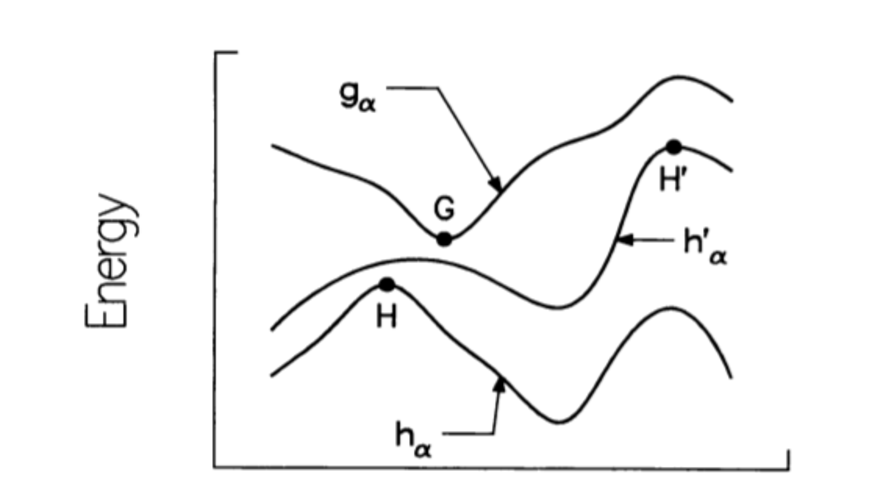
\includegraphics[width=0.8\textwidth]{pics/gold1.pdf}
    \caption{Rotamer $g_\alpha$ has a min of G, while rotamer $h_\alpha$ has max of H. So $g_\alpha$ can be eliminated using original DEE criterion. But original DEE is not able to prune rotamer $h'_{\alpha}$ whereas Goldstein is able to because it compares the minimum of the gap between the functions $g_\alpha$ and $h'_\alpha$.Figure from~\cite{Goldstein1994}.}
    \label{fig:goldstein}
\end{figure}

\pagebreak

\subsection{General Goldstein}
The general Goldstein criteria compares the average of the energies contributions from the neighbours instead of using max, min methods. This is believed to be even more powerful but may be difficult to implement. If this condition holds it means that there must exist a rotameric configuration $r_i^r$ that has better energy than $r_i^A$.
\[
E_i(r_i^A)-\sum_{r=1}^R C_r E_i(r_i^r) + \sum_j \min_X \left( E_{ij}(r_i^A,X) - \sum_r C_rE_{ij}(r_i^A,X) \right) >0
\]
such that $C_r \geq 0$ and $\sum_r C_r=1$. See Figure~\ref{fig:goldstein_gen} for an illustration of the generalized goldstein criteria intuition. 

 A doubt remains as to how to pick $C_r$? While any value of $C_r$ would work, which one would you pick to get maximum eliminatory power? This has been elaborated by~\cite{Lasters1995} who use a linear programming approach in order to find the optimal value of $C_r$. But a problem remains that even on finding the optimal value,e ven if there exists one candidate whose energy is greater than the rotamer under elimination consideration then it increases the average energy of the ensemble for that conformation.

\begin{figure}[h!]
    \centering
    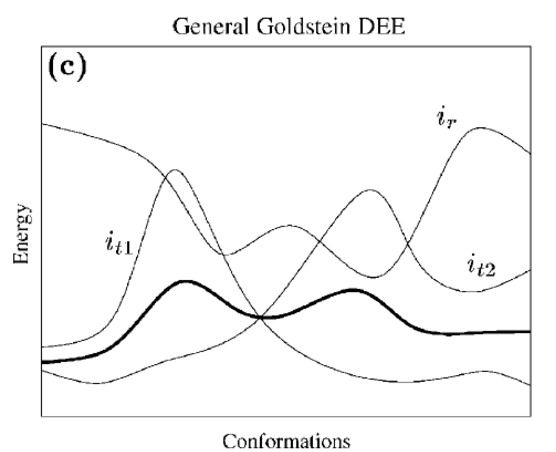
\includegraphics[width=0.7\textwidth]{pics/goldgen.pdf}
    \caption{Rotamer $i_r$ cannot be eliminated by either of the rotamers $i_{t1}$ or $i_{t2}$ since they are greater than $i_r$ for some conformation. However the average of the two taken together $C_r=0.5$ is lower than the $i_r$ everywhere, so this is able to eliminate $i_r$.  Figure reproduced from~\cite{Pierce2000}}
    \label{fig:goldstein_gen}
\end{figure}

\pagebreak

\subsection{Singles Goldstein Implementation}
The psuedo-code for one round of singles goldstein is presented. The energy values for the unit and pairwise terms have been pre-computed. The complexity of this algorithm is $O(n^2r^3)$. 

\begin{algorithm}
\caption{Singles Goldstein DEE} \label{algo:goldstein}
\begin{algorithmic}
\For{each position $i$}
	\For{each rotamer $r$ at $i$}
		\For{each candidate rotamer $t$ at $i$}
			\State $X \gets E_i(r_i^r) - E_i(r_i^t)$
			\ForAll{positions $j \not= i$} 
				\ForAll{rotamers $u$ at position $j$}
					\State $Y = \min_u\left[E_{ij}(r_i^r,r_j^u) - E_{ij}(r_i^t,r_j^u) \right]$
				\EndFor
				\State $X \gets X + Y$
			\EndFor
			\If{$X>0$}
				\State eliminate $r_i^r$
				\State break
			\EndIf
		\EndFor
	\EndFor
\EndFor
\end{algorithmic}
\end{algorithm}

\pagebreak


\subsection{Renormalized residues}
Renormalizing residues refers to the concept of grouping residues together and treating them as one unit. It is similar to the notion of forming cliques in a graphical model. So if in the original model residue $i$ and $j$ had $c$ rotamers each, in the renormalized super-residue it will have $c^2$  rotamers. Applying Singles DEE to this super node is the same as pairwise DEE to non-renormalized model. This can be extended to groups of multiple residues not just pairs. In principle one can bunch all residues together and have to solve the original problem but using way more space. 


\subsection{Goldstein Discussion}
Despite all the DEE stuff, the author mentions that interaction energy cutoffs is really an effective way to first prune the search space. This is an example of where aesthetic purity might be overriden for practical effectiveness. The DEE pruning criteria is rarely powerful enough to be able to find the GMEC, but it reduces the search space enought so that one can apply other techniques such as MCMC to find a reasonably good solution. 
\\
\\
While designing DEE experiments that preserve the GMEC, it is not necessary to prove the effectiveness of your algorithm with respect to how it performs on real protein structures in terms of RMSD. This is because DEE finds the GMEC, so whatever artefacts you might see are due to the force field. 
\\
\\
The goldstein paper also has a discussion about spin glasses which are nothing but ising models. They contain random pairwise energy values, but otherwise have the same formulation as the SCP problem. The author observes that the DEE method is not that effective in pruning spin glasses when compared to proteins side chains. He suggests that this might be due to the folding funnel of proteins.

\section{Split DEE}
The split DEE(sDEE) is a stronger criterion that can be used to further prune the search space \cite{Pierce2000}. This can be used when the goldstein criteria can no longer identify any more dead-ends. sDEE splits the solution space into partitions and then runs Goldstein DEE in each of these partitions. If Goldstein DEE is able to eliminate a rotamer $r_i^A$ from each of these partitions then we can remove $r_i^A$ from the whole space. Once some rotamers have been removed using sDEE, Goldstein singles and pairs DEE can again be applied iteratively in order to prune out more of the search space. The split DEE criterion has a singles as well as a general version. The singles sDEE criterion splits on one residue only. We split on each $r_k^v$ where $r_k^v \in r_k$, the rotamer space of residue $k$. An illustration of the splitDEE criterion is provided in Figure~\ref{fig:splitDEE}. The singles sDEE criterion states that $r_i^A$ can be eliminated if $\exists$ a $r_i^B$ for every partition of $r_k^v$ such that the following condition holds: 

\begin{equation}
\label{eqn:sDEE_singles}
\begin{split}
E_i(r_i^A) - E_i(r_i^B) &+ \sum_{j\neq i \neq k} \min_X \left(E_{ij}(r_i^A,r_j^X)-E_{ij}(r_i^B,r_j^X) \right)\\
&+ \left[E_{ik}(r_i^A,r_k^v)-E_{ik}(r_i^B,r_k^v)\right] > 0 
\end{split}
\end{equation}
The residue k is over all residue positions $k \in \{1,\dots, n\}\backslash i$. The computational cost of the singles sDEE criterion is $O(n^2r^3)$ which is the same as the singles goldstein criteria. Naively, it might appear that the cost is $O(n^2r^4)$ because of the additional residue $k$. However it can be avoided if the implementation is done a little cleverly by storing computations. We will present the algorithm that gives this bound. 

\subsection{General Split DEE}
The general sDEE criterions allows splits on more than one residue. Suppose we split on s residues such that $k \in \{k_1,\dots,k_s\}$, the general sDEE criteria becomes :
\begin{equation}
\label{eqn:sDEE_gen}
\begin{split}
E_i(r_i^A) - E_i(r_i^B) &+ \sum_{j\neq i \neq k_1\dots k_s} \min_X \left(E_{ij}(r_i^A,r_j^X)-E_{ij}(r_i^B,r_j^X) \right)\\
&+ \sum_{k=k_1\dots k_s}\left[E_{ik}(r_i^A,r_k^v)-E_{ik}(r_i^B,r_k^v)\right] > 0 
\end{split}
\end{equation}

The residue $k_1\dots k_s$ is over all $n-1 \choose s$ sets of residues . The computational cost of the general split DEE quickly becomes exponential in the number of splits.  It is not feasible to use the general sDEE for more than a few splits. In particular for $s$ splits, the cost is $O(r^{2+s}nq)$  where q is the number of ways of choosing $s$ splits from $n-1$ residues.
\[
q = \frac{(n-1)!}{s!(n-1-s)!}
\]
It decomposes as $nr^2(n-s)r + nr{n\choose s}r(n-s)$. This answers two FAQs about sDEE. 
\begin{enumerate}
\item How many splits to choose? - s
\item How to pick which position to split on ? - Iterate over all $n-1 \choose s$
\end{enumerate}

\begin{figure}[h!]
    \centering
    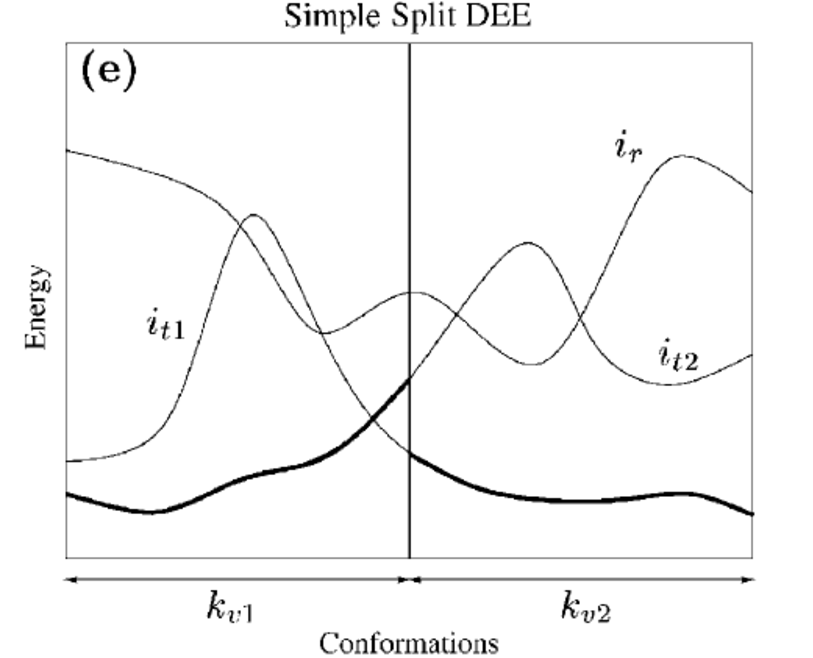
\includegraphics[width=0.7\textwidth]{pics/split1.pdf}
    \caption{Rotamer $i_r$ cannot be eliminated by either of the rotamers $i_{t1}$ or $i_{t2}$ since they are greater than $i_r$ for some conformation. However if the conformation space is split into two halves as shown by the vertical line, then it is possible to eliminate $i_r$ from each of the partitions. Figure reproduced from~\cite{Pierce2000}}.
    \label{fig:splitDEE}
\end{figure}
\pagebreak

\subsection{Magic Bullet Splitting}
The concept of Magic Bullet~\cite{Gordon1998} Doubles was introduced as a technique for speeding up the calculations for pairs elimination criteria for DEE. They used this to (1) reduce computational cost to $O(n^3r^4)$ down from $O(n^3r^5)$ that is normally needed for Goldstein doubles (2) Increase the elimination power by 20\% to 60\% if using the same $O(n^3r^5)$ complexity. 
\\
\\
The authors of sDEE developed a version of magic bullet for choosing exactly one of the $n-1 \choose s$ possible $k_1\dots k_s$ split points as the magic bullet split point. This would reduce complexity from $O(r^{2+s}nq)$ to $O(r^{2+s}n)$, effectively getting rid of the $O(q)$ term. Intuitively, the best splitting locations should be those that have the best strong interactions with $r_i$. They use the following metric to rank the possible split points which basically says that there is a significant energy difference between $r_i^A$ and $r_i^B$ when the split residue $r_k$ is used. 
\[
\text{Score}_1 = \min_k \min_B \min_v[E(r_i^Ar_k^v) - E(r_i^Br_k^v)]
\]

Is this is a better a scoring metric ? 
\[
\text{Score}_2 = \max_k \max_B \max_v \left( \left| E(r_i^Ar_k^v) - E(r_i^Br_k^v) \right| \right)
\]

For $s=2$ splits they call the split as $s=2_{mb}$ and this has a $O(r^4n)$ cost which is only a factor $O(r/n)$ cost more than the full $s=1$ singles sDEE of $O(n^2r^3)$. 

\subsection{Singles Split DEE Implementation}

\begin{algorithm}
\caption{The simple split DEE} \label{algo:sDEE}
\begin{algorithmic}
\For{each position $i$}
	\For{each rotamer $r$ at $i$}
		\For{each candidate rotamer $t$ at $i$}
			\ForAll{positions $j\not= i$}
				\ForAll{rotamers $u$ at position $j$}\
					\State $Y_{jt} \gets \min_u\left[E_{ij}(r_i^r,r_j^u) - E_{ij}(r_i^t,r_i^u)\right]$
				\EndFor
			\EndFor
		\EndFor
		\For{each splitting position $k$}
			\State $elim_v \gets false \quad \forall v$ at $k$
			\For{each competitor $t$ at $i$}
				\State $X \gets E_i(r_i^r) - E_i(r_i^t)$
				\ForAll{other positions $j$, $j\not=i\not=k$}
					\State $X \gets X + Y_{jt}$
				\EndFor
				\For{each partition $v$ at $k$}
					\If{$X+\left[E_{ik}(r_i^r,r_k^v) - E_{ik}(r_i^t,r_k^v)\right] > 0$}
						\State $elim_v \gets true$						
					\EndIf
				\EndFor
			\EndFor
			\If{$elim_v == true \quad \forall v$ at $k$} 
				\State eliminate $r_i^r$ and break
			\EndIf
		\EndFor
	\EndFor
\EndFor
\end{algorithmic}
\end{algorithm}

\pagebreak

All of the unit and pairwise energy terms are precomputed before the DEE algorithm is applied. The key point of the implementation to save compute cost is that the minima over $u$ must be computed prior to splitting over $k$ to avoid higher complexity due to nesting. 
\\
\\
The residue k is over all residue positions $k \in \{1,\dots, n\}\backslash i$. With this algorithmic implementation the computational cost is $O(n^2r^2(n+r))$. For most sequence design applications $n \sim r$ or $n\ll r$, so the complexity can be written as $O(n^2r^3)$ same as that of the goldstein criteria. The authors claim that this particular implementation is tailored towards protein design applications so that it favors $n \ll r$ calculations. This does not make sense since we are getting a $O(n^2r^3)$ complexity, wouldn't it better to have $O(n^3r^2)$ ? They say that they can change the loop structure for homology modeling applications where it $n \gg r$. 
\\
\\
The following DEE cycle can be used prune the maximum. All steps included is called the Magic Bullet2 sDEE. Eliminating step 3 is singles sDEE. Eliminating steps 2 and 3 is the original Goldstein DEE. 
\begin{enumerate}
\item Simple Goldstein Singles DEE until no further elimination
\item Simple split Singles DEE until no further elimination
\item Magic Bullet2 split DEE once for each rotamer
\item Alternate sequentially between the following applying one during each cycle
\begin{enumerate}
\item  Fast Goldstein doubles calculations to flag dead-ending pairs
\item Goldstein doubles calculations to flag dead-ending pairs
\item Unification of two residues with highest fraction of dead-ending pairs
\end{enumerate}
\item Return to 1
\end{enumerate}


\subsection{Bottom Line DEE}
We present the Bottom line DEE technique as it is theoretically interesting and is closely related to split DEE. It has the most eliminating power. However it is not possible to implement it in practice as it involves taking a minimum over energies over all rotamers of all neigbhors of the residue under consideration, a $O(r^n)$ calculation.  The main idea is that it is not necessary for the same rotamer $r_i^B$ to eliminate the rotamer $r_i^A$ at all conformations of the neighbours. It is merely sufficient for there to exist some candidate rotamer that is able to eliminate the rotamer $r_i^A$ under consideration. An illustration of the Bottom Line DEE is shown in Figure~\ref{fig:bottomDEE}.

\begin{figure}[h!]
    \centering
    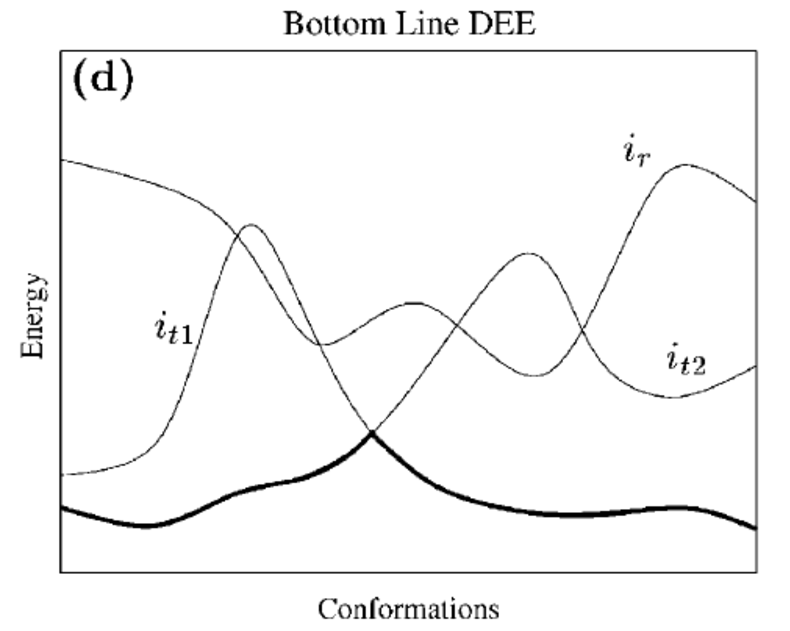
\includegraphics[width=0.7\textwidth]{pics/bottom.pdf}
    \caption{Rotamer $i_r$ cannot be eliminated by either of the rotamers $i_{t1}$ or $i_{t2}$ since they are greater than $i_r$ for some conformation. However the minimum of the two taken together is lower than the $i_r$ everywhere, so this is able to eliminate $i_r$. Unfortunately, though theoretically appealing it is not possible to compute this minimum value efficiently in practice since it takes $O(r^n)$ in practice. Figure reproduced from~\cite{Pierce2000}}.
    \label{fig:bottomDEE}
\end{figure}

\pagebreak

\subsection*{Split DEE discussion}
The authors in~\cite{Pierce2000} claim that this particular implementation is tailored towards protein design applications so that it favors $n \ll r$ calculations. This does not make sense since we are getting a $O(n^2r^3)$ complexity, wouldn't it better to have $O(n^3r^2)$ ?


\section{Other DEE related}
This section covers a number of other related DEE work that came about contemporarily and after the initial DEE work. Some of them further develop the core DEE criterion and some others make novel modifications that make the algorithm applicable to novel applications. 


\subsection{DEE for Protein Design- Mayo}
DEE can also be used for sequence design and this was first shown by Dahiyat et.al~\cite{Dahiyat1997}. They considered the problem of de-novo designing a novel sequence that fit onto a particular scaffold. They proposed to design a $\beta\beta\alpha$ motif that is normally found in the Zif268 protein. 
From a biological perspective this domain is interesting, since it has $\beta$ sheets, $\alpha$ helices and loop regions. The domain is small enough so that it does not have an extensive core. 
This fact is important since earlier attempts at protein redesign have been focused on the protein core only. 
They make an important observation about the important of the energy function. It depends on the region of the protein to determine the energy function. The hydrophobic region, the surface area and the boundary regions have different dependences on H-bonds, solvation effect, van der waal effects. 
They incorporate these favtors into the energy function. 
\\
\\
Their sequence redesign problem had 28 residues. They restricted the state space of amino acids depending on whether it was hydrophobic, present on the surface etc. Still they had a net sequence space of $1.9 \times 10^{27}$. To get a handle on this size, they point that a single molecule peptide library enumerating this space would weight 11.6 tonnes. They further point that in order to do DEE, one needs to consider the rotamers of the side chain and this net space comes to about $1.1 \times 10^{62}$ possible rotamers. 
Their DEE implementation on this problem took 90 CPU hours to compute. They called their GMEC seq FSD1. They claimed that FSD1 was quite novel as it did not match any other sequences from BLAST searches. Random MCMC searches showed a dense search space around FSD1, implying that some of the sequences had low energy. 
Finally, they were able to demonstrate the efficacy of FSD1 conclusively by doing NMR and showing that the FSD1 structure was in close agreement with Zif268.

\subsection{Gordon Criteria}



\subsection{DEE/A*}

\subsection{Branch and Terminate}

\subsection{K*??} 

\section{Newer Methods}

\subsection{DEE for Multistate protein design}
A subproblem in the 

\subsection{DEE for Flexible backbone}

\subsection{minDEE/K*}

\subsection{restricted DEE - Lilien}

\subsection{iminDEE - Continuous rotamers}

\subsection{Backrub}

\subsection{BroMAP}

\subsection{DEEPer}

\subsection{Ensemble K*}

\section{Connections}
\subsection{Graphical models and Max Product BP}

\subsection{Dynamic Programming}


\section{Implementation}
Calculation  of $E_i(r_i)$ and $E_{ij}(r_i,r_j)$ can be quite expensive and is usually the major cost while applying the DEE procedure. However they scale linearly and quadratically with respect to rotamer size respectively, but just with large constants. 

First the method checks all rotamers for every amino acid and flags them. Then it checks rotamer pairs. This process iterates until no more rotamers or pairs can be eliminated. 

In practice, the number of rotamers can be reduced significantly by applying some screening rules. Pre-screening rotamers that cause clashes and have energy more than 30kcal/mol with backbone and surrounding side chains can be eliminated. Desmet et.al~\cite{Desmet1992} report  that they were able to achieve 44\% and 6\% of the rotamers in their experiment were eliminated based on backbone and side chain clashes thresholding respectively. This meant a reduction of the search space from $2.7\times10^{76}$ to $6.2\times10^{53}$ rotamer conformations. This is quite a large saving. After six iterations of DEE the solution space was reduced to $10,800$. They could easily brute force this. 

One way to speed up calculations for DEE is to pre-cache the min and max value of the energy matrices into vectors while doing the energy calculations themselves. This can prevent repeated min and max calculations while using a little extra memory. Supposing there are $n$ residues and $r$ rotamers per residue then you should not need $O(n^2r)$ space by pre-caching $\min_X E_{ij}(r_i^A,r_j^X)$.

Parallelization of DEE calculations using MPI on different clusters or even using GPUs can be explored. 

\subsection{Space requirements}
The space needed to store the energy values can be a limiting factor for large sequences. Let $N$ be the number of amino acids in the protein and $R$ be the number of rotamers per amino acid. Then we need $O(NR)$ space for unit energy values and $O(N^2R^2)$ for the pairwise energy values. 

\section{Discussion}

Problems with DEE :
\begin{itemize}
\item Is it worth trying to find the GMEC given that energy functions are not that accurate in the first place?
\item Is DEE a dual of Dynamic programming ? 
\item How are the energies pre-computed ? What is the conmplexity of doing this ?
\item How do the space requirements compare with the time requirements ?
\item How does the algo scale with size of the system ? Are some large systems impossible to model using this method ? 
\item How does DEE compare with other non-DEE techniques such as Monte Carlo, etc..
\item When calculating $E(r)$ the energy of the whole protein are all pairs of energies evaluated or is some sort of distance constraint enforced ?
\item Should you use bbdep rotamers or bbindep rotamers ?
\item What is the connection between local optimality of GMEC to graphical models and max product
\end{itemize}

\section{New Ideas}

\begin{itemize}
\item Is this is a better a scoring metric for magic bullet splitting in  \cite{Pierce2000} ? 
\[
\text{Score}_2 = \max_k \max_B \max_v \left( \left| E(r_i^Ar_k^v) - E(r_i^Br_k^v) \right| \right)
\]
\item For sequence redesign there is usually a prior step wherein they prune the state spaces of some amino acids based on whether it is hydrophobic/etc. Is there a more principled way to do this so that the elimination happens during the algorithm stage ?
\end{itemize}




\pagebreak
\newpage

\appendix


\section{Datasets used}


\begin{center}
    \begin{tabular}{ | p{3cm} | p{3cm} | p{6cm} |}
    \hline
    \textbf{Paper} & \textbf{Dataset} & \bf{Summary} \\ \hline
    Desmet1992, Original DEE~\cite{Desmet1992} & Insulin, haemocyanin & Compared agreement with pdb for Insulin. Predicted on blind study of haemocyanin \\ \hline
    Goldstein1994, Original Goldstein~\cite{Goldstein1994} & apo-myogloblin, lysosome, 7LZM, 5MBA& Showed parameter reduction, compute time. Randomly perturbed energy functions and compared to spin glasses. \\ \hline
Pierce2000, split DEE~\cite{Pierce2000} & Plastocyanin(2PCY), Gprotein(1PGA), Gprotein $\beta$-sheet& Showed parameter reduction,time using Goldstein, sDEE, MB2 sDEE for each test case. Core easier to prune than surface. \\ \hline
    Tuesday & 9C & Cloudy with rain, across many northern regions. Clear spells
    across most of Scotland and Northern Ireland,
    but rain reaching the far northwest. \\ 
    \hline
    \end{tabular}
\end{center}


\section{Multistate DEE}
DEE solves a discrete combinatorial optimization problem. The main contribution of the DEE algorithm is that it reduces the search space by provably pruning out some candidates. However it has to make sure that whne pruning out candidates it still preserves the GMEC. For it to be able to do this it needs to make some assumptions about the form of the energy function. 

For single state protein design the optimization problem is  : 
\[
S^* = \argmin_S E^*(S) = \argmin_S \left( \min_r E(r,S) \right)
\]

For multistate it is :
\[
S^* = \argmin_S E^*_1(S) + E^*_2(S) = \argmin_S\left( \min_r E_1(r,S) + \min_r E_2(r,S)\right)
\]

Multistate protein design tries to find the sequence that is stable under a number of different states. In their method yhey use the type-dependent DEE for pruning out the space of candidate solutions, while preserving the GMEC. Multistate optimization falls into two categories. First, wherein you are trying to design a structure that is stable in multiple state and second wherein you are trying to design for specificity which means that you are trying to design a sequence that is stable in one state but unstable in other states. The canonical way to represent the multistate optimization for specificity is :
\[
\begin{split}
Score(S) &= \alpha E_{pos}^*(S) - \beta E_{neg}^*(S) \quad \text{where } \alpha,\beta \geq 0 \\
S^* & = \argmin_S \left[\alpha \min_{\tau(r)=S} E_{pos}(r_{pos}) - \min_{\tau(r)=S} \beta E_{neg}(r_{neg})) \right]
\end{split} 
\]

Note that $E_{pos}^*(S)$ denote the minimal energy conformation for a particular sequence. I am confused isn't finding this exponentially hard as well ? Because we proved previously that the side chain optimization problem is NP hard. The way seqeunce design works with DEE is that the sequence space is expanded to include the rotameric space as well. So instead of doing DEE on a $20^N$ space you perform DEE over a $(20*n_{rot})^N$ space. Whatever the optimal rotamer assignments are, you can calculate the optimal sequence by just mapping the rotamer to the appropriate sequence. 
\\
\\
One strategy to do multistate design could be to combine the rotameric spaces of the two states and then optimize that energy function. Such as  : 
\[
\tilde{E_{ij}}(r_i,r_j) = \alpha E_{pos_{ij}}(r_i,r_j) - \beta E_{neg_{ij}}(r_i,r_j)
\]
However, this scheme assumes that the both states will have the same rotameric states. However, we want to do the minimization over the sequence space while letting the rotamers be different in each state. 



\bibliographystyle{plain}
\bibliography{refs}


\end{document}